%!TEX root = ../Theory.tex

\section{Reflectometry} % (fold)
\label{sec:reflectometry}

The propagation of light as a magneto-electric wave of wave vector $\vb{k}$ is given by,
\begin{align*}
	\vb{E}\pqty{\vb{r},t} &= \vb{E}_{0}e^{i\pqty{\vb{k}\cdot\vb{r} - \omega t}} & \vb{B}\pqty{\vb{r},t} &= \frac{\vu{k}\times\vb{E}\pqty{\vb{r},t}}{v}
\end{align*}

\begin{align*}
	\vb{E}\pqty{\vb{r},t} &= \vb{E}_{0}e^{i\pqty{\vb{k}\cdot\vb{r} - \omega t}} & \omega \vb{B}\pqty{\vb{r},t} &= \vb{k}\times\vb{E}\pqty{\vb{r},t}
\end{align*}

In each layer $j$, there is a wave probagating from the incidence side, and a reflected wave,
\begin{align*}
	\vb{E}_j\pqty{\vb{r},t} &= 
		\vb{E}_{0j}^{(I)}e^{i\pqty{\vb{k}_j^{(I)}\cdot\vb{r} - \omega t}} + 
		\vb{E}_{0j}^{(R)}e^{i\pqty{\vb{k}_j^{(R)}\cdot\vb{r} - \omega t}} \\
	\omega\vb{B}_j\pqty{\vb{r},t} &= 
		\vb{k}_j^{(I)}\times\vb{E}_{0j}^{(I)}e^{i\pqty{\vb{k}_j^{(I)}\cdot\vb{r} - \omega t}} + 
		\vb{k}_j^{(R)}\times\vb{E}_{0j}^{(R)}e^{i\pqty{\vb{k}_j^{(R)}\cdot\vb{r} - \omega t}}
\end{align*}

Wave vector and group speed are related,
\begin{align*}
	k_j^{(I,R)}v_j &= \omega & k_j^{(I,R)} = \abs*{\vb{k}_j^{(I,R)}}
\end{align*}

\begin{align*}
	n_j v_j &= c & \frac{n_j}{k_j^{(I,R)}} &= \frac{c}{\omega} = \frac{\lambda}{2\pi}
\end{align*}

% \begin{align*}
% 	\vb{E}_{j-1}\pqty{\vb{r}_j,t} &= \vb{E}_{j}\pqty{\vb{r}_j,t} \\
% 	\vb{B}_{j-1}\pqty{\vb{r}_j,t} &= \vb{B}_{j}\pqty{\vb{r}_j,t}
% \end{align*}

\begin{figure}
\begin{center}
    {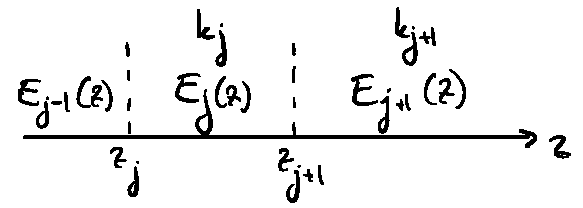
\includegraphics{Figures/SpaceDiscretion.pdf}
    }
\caption{
Caption
}
\label{fig:1}
\end{center}
\end{figure}

The interface between layer $j-1$ and $j$ is define as $\boldsymbol{\mathsf{r}}_j$. 
\begin{align*}
	\boldsymbol{\mathsf{r}}_j = x\vu{x} + y\vu{y} + z_j\vu{z}
\end{align*}
The electric field component at the interface need to respect the following equation
\begin{align*}
	\pqty{\vb{E}_{j-1}\pqty{\boldsymbol{\mathsf{r}}_j,t}}_{x,y} &= \pqty{\vb{E}_{j}\pqty{\boldsymbol{\mathsf{r}}_j,t}}_{x,y} \\
	\epsilon_{j-1}\pqty{\vb{E}_{j-1}\pqty{\boldsymbol{\mathsf{r}}_j,t}}_z &= \epsilon_{j}\pqty{\vb{E}_{j}\pqty{\boldsymbol{\mathsf{r}}_j,t}}_z
\end{align*} while the magnetic field components,
\begin{align*}
	\frac{1}{\mu_{j-1}}\pqty{\vb{B}_{j-1}\pqty{\boldsymbol{\mathsf{r}}_j,t}}_{x,y} &= \frac{1}{\mu_j}\pqty{\vb{B}_{j}\pqty{\boldsymbol{\mathsf{r}}_j,t}}_{x,y} \\
	\pqty{\vb{B}_{j-1}\pqty{\boldsymbol{\mathsf{r}}_j,t}}_z &= \pqty{\vb{B}_{j}\pqty{\boldsymbol{\mathsf{r}}_j,t}}_z 
\end{align*}

All these equation will have phase factors that must connect at the interface. 
\begin{align*}
	e^{i\pqty{\vb{k}_j^{(I,R)}\cdot\boldsymbol{\mathsf{r}}_j - \omega t}} = e^{-i\omega t}\exp i\pqty{k^{(I,R)}_{x,j}x + k^{(I,R)}_{y,j}y + k^{(I,R)}_{z,j}z_j}
\end{align*}

The $x$ and $y$ dependance must be the same on each side of each equation, meaning that, in each layer we must have
\begin{align*}
	k_{x,j} &= k^{(I)}_{x,j} = k^{(R)}_{x,j} & k_{y,j} &= k^{(I)}_{y,j} = k^{(R)}_{y,j} & k_{z,j} &= k^{(I)}_{z,j} = -k^{(R)}_{z,j}
\end{align*} and between planes
\begin{align*}
	k_{x,j-1} &= k_{x,j} & k_{y,j-1} &= k_{y,j}
\end{align*}

If we define $\theta_j$ as the angle between the interface and $\vb{k}_j$, we get the following relations (Snell's law).
\begin{align*}
	k_{j-1}\cos\theta_{j-1} &= k_{j}\cos\theta_{j} & \frac{\cos\theta_j}{\cos\theta_{j-1}} &= \frac{k_{j-1}}{k_j} = \frac{n_{j-1}}{n_j} = \pqty{\frac{\epsilon_{j-1}\mu_{j-1}}{\epsilon_j\mu_j}}^{1/2}
\end{align*}

If the first incident beam is $k_0$ at an angle $\theta_0$, this means,
\begin{align*}
	k_{0}\cos\theta_{0} &= k_{j}\cos\theta_{j} & \frac{k_0}{n_0} &= \frac{k_j}{n_j}
\end{align*}



% \begin{align*}
% 	\epsilon_{j-1}\pqty{E^{(I)}_{0z,j-1}e^{ik^{(I)}_{z,j-1}z_j} + E^{(R)}_{0z,j-1}e^{ik^{(R)}_{z,j-1}z_j}} &= 
% 	\epsilon_{j}\pqty{E^{(I)}_{0z,j}e^{ik^{(I)}_{z,j}z_j} + E^{(R)}_{0z,j}e^{ik^{(R)}_{z,j}z_j}} \\
% 	E^{(I)}_{0x,y,j-1}e^{ik^{(I)}_{z,j-1}z_j} + E^{(R)}_{0x,y,j-1}e^{ik^{(R)}_{z,j-1}z_j} &= 
% 	E^{(I)}_{0x,y,j}e^{ik^{(I)}_{z,j}z_j} + E^{(R)}_{0x,y,j}e^{ik^{(R)}_{z,j}z_j}
% \end{align*}

Polarisation in plane, with $k_y = 0$,
\begin{align*}
	E^{(I)}_{0x,j} &= E^{(I)}_{0,j}\sin\theta_j & E^{(R)}_{0x,j} &= -E^{(R)}_{0,j}\sin\theta_j \\
	E^{(I)}_{0y,j} &= 0 & E^{(R)}_{0y,j} &= 0 \\
	E^{(I)}_{0z,j} &= E^{(I)}_{0,j}\cos\theta_j & E^{(R)}_{0z,j} &= E^{(R)}_{0,j}\cos\theta_j
\end{align*}

\begin{align*}
	B^{(I)}_{0x,j} &= 0 & B^{(R)}_{0x,j} &= 0 \\
	\omega B^{(I)}_{0y,j} &= k^{(I)}_jE^{(I)}_{0,j} & \omega B^{(R)}_{0y,j} &= k^{(R)}_jE^{(R)}_{0,j} \\
	B^{(I)}_{0z,j} &= 0 & B^{(R)}_{0z,j} &= 0 \\
\end{align*}

The relevant equations are
\begin{align*}
	\sin\theta_{j-1}\pqty{E^{(I)}_{0,j-1}e^{ik_{z,j-1}z_j} + E^{(R)}_{0,j-1}e^{-ik_{z,j-1}z_j}} &=
	\sin\theta_{j}\pqty{E^{(I)}_{0,j}e^{ik_{z,j}z_j} - E^{(R)}_{0,j}e^{-ik_{z,j}z_j}} 
	\\
	\epsilon_{j-1} \cos\theta_{j-1} \pqty{E^{(I)}_{0,j-1}e^{ik_{z,j-1}z_j} + E^{(R)}_{0,j-1}e^{-ik_{z,j-1}z_j}} &=
	\epsilon_{j} \cos\theta_{j} \pqty{E^{(I)}_{0,j}e^{ik_{z,j}z_j} + E^{(R)}_{0,j} e^{-ik_{z,j}z_j}} 
	\\
	\frac{k_{j-1}}{\mu_{j-1}}\pqty{E^{(I)}_{0,j-1} e^{ik_{z,j-1}z_j} + E^{(R)}_{0,j-1} e^{ik_{z,j-1}z_j}} &=
	\frac{k_{j}}{\mu_{j}}\pqty{E^{(I)}_{0,j} e^{ik_{z,j}z_j} + E^{(R)}_{0,j} e^{ik_{z,j}z_j}}
\end{align*}

The third one is equivalent to the second one.

\begin{align*}
	\vb{W}_j \equiv \vb{S}_j\pqty{z}\cdot\vb{E}_j
\end{align*} where
\begin{align*}
	\vb{W}_j\pqty{\vb{r}} &= \pmqty{E_{0x,j}\pqty{\vb{r}} \\ \epsilon_j E_{0z,j}\pqty{\vb{r}}} = E_{0,j}\pqty{\vb{r}}\pmqty{\sin\theta_j \\ \epsilon_j \cos\theta_j}
	&\vb{E}_j &= \pmqty{E_{0,j}^{(I)} \\ E_{0,j}^{(R)}} 
	& 
	\vb{S}_j\pqty{z} &= \pmqty{
		\alpha_j e^{ik_{z,j}z} & 
		-\alpha_j e^{-ik_{z,j}z} \\
		\beta_j e^{ik_{z,j}z} & 
		\beta_j e^{-ik_{z,j}z}}
\end{align*} where we defined
% \begin{align*}
% 	\epsilon_j\cos\theta_j = \frac{n_j^2}{\mu_j}\cos\theta_j = \frac{\lambda n_j k_j}{\mu_j}\cos\theta_j
% \end{align*}
% \begin{align*}
% 	\frac{n_{j-1}}{\mu_{j-1}} \pqty{E^{(I)}_{0,j-1}e^{ik_{z,j-1}z_j} + E^{(R)}_{0,j-1}e^{-ik_{z,j-1}z_j}} &=
% 	\frac{n_{j}}{\mu_{j}} \pqty{E^{(I)}_{0,j}e^{ik_{z,j}z_j} + E^{(R)}_{0,j} e^{-ik_{z,j}z_j}} \\
% 	\pqty{1 - \frac{n_0^2\cos^2\theta_0}{n_{j-1}^2}}^{1/2}\pqty{E^{(I)}_{0,j-1}e^{ik_{z,j-1}z_j} + E^{(R)}_{0,j-1}e^{-ik_{z,j-1}z_j}} &=
% 	\pqty{1 - \frac{n_0^2\cos^2\theta_0}{n_{j}^2}}^{1/2}\pqty{E^{(I)}_{0,j}e^{ik_{z,j}z_j} + E^{(R)}_{0,j}e^{-ik_{z,j}z_j}}
% \end{align*}
% \begin{align*}
% 	E^{(I)}_{0,j-1}e^{ik_{z,j-1}z_j} + E^{(R)}_{0,j-1}e^{-ik_{z,j-1}z_j} &=
% 	\frac{\epsilon_j}{\epsilon_{j-1}}\frac{\cos\theta_j}{\cos\theta_{j-1}} \pqty{E^{(I)}_{0,j}e^{ik_{z,j}z_j} + E^{(R)}_{0,j} e^{-ik_{z,j}z_j}}  
% 	% \\
% 	% E^{(I)}_{0,j-1} e^{ik_{z,j-1}z_j} + E^{(R)}_{0,j-1} e^{ik_{z,j-1}z_j} &=
% 	% \frac{k_{j}}{k_{j-1}}\frac{\mu_{j-1}}{\mu_{j}}\pqty{E^{(I)}_{0,j} e^{ik_{z,j}z_j} + E^{(R)}_{0,j} e^{ik_{z,j}z_j}}
% \end{align*}
\begin{align*}
	\alpha_j &\equiv \sin\theta_j = \pqty{1 - \frac{n_0^2\cos^2\theta_0}{n_{j}^2}}^{1/2} & \beta_j &\equiv \epsilon_j\cos\theta_j  = \frac{n_j}{\mu_j} \lambda k_0 \cos\theta_0
\end{align*}so that,
\begin{align*}
	\vb{W}_{j-1}\pqty{\boldsymbol{\mathsf{r}}_j,t} &= \vb{W}_{j}\pqty{\boldsymbol{\mathsf{r}}_j,t}
\end{align*}

\begin{align*}
	\det{\vb{S}_j} &= 2\alpha_j\beta_j = 2\epsilon_j\sin\theta_j\cos\theta_j = 2n^2_j\sin\theta_j\cos\theta_j = 2n_j\sin\theta_j n_0\cos\theta_0
\end{align*}

Polarisation out of plane, with $k_y = 0$,
\begin{align*}
	E^{(I)}_{0x,j} &= 0 & E^{(R)}_{0x,j} &= 0 \\
	E^{(I)}_{0y,j} &= E^{(I)}_{0,j} & E^{(R)}_{0y,j} &= E^{(R)}_{0,j} \\
	E^{(I)}_{0z,j} &= 0 & E^{(R)}_{0z,j} &= 0 \\
\end{align*}

\begin{align*}
	\omega B^{(I)}_{0x,j} &= k_j E^{(I)}_{0,j}\sin\theta_j & \omega B^{(R)}_{0x,j} &= -k_j E^{(R)}_{0,j}\sin\theta_j \\
	B^{(I)}_{0y,j} &= 0 & B^{(R)}_{0y,j} &= 0 \\
	\omega B^{(I)}_{0z,j} &= k_j E^{(I)}_{0,j}\cos\theta_j & \omega B^{(R)}_{0z,j} &= k_j E^{(R)}_{0,j}\cos\theta_j \\
\end{align*}

The relevant equations are
\begin{align*}
	E^{(I)}_{0,j-1}e^{ik_{z,j-1}z_j} + E^{(R)}_{0,j-1}e^{-ik_{z,j-1}z_j} &=
	E^{(I)}_{0,j}e^{ik_{z,j}z_j} + E^{(R)}_{0,j} e^{-ik_{z,j}z_j}
	\\
	k_{j-1}\sin\theta_{j-1}\pqty{E^{(I)}_{0,j-1}e^{ik_{z,j-1}z_j} + E^{(R)}_{0,j-1}e^{-ik_{z,j-1}z_j}} &=
	k_{j}\sin\theta_{j}\pqty{E^{(I)}_{0,j}e^{ik_{z,j}z_j} - E^{(R)}_{0,j}e^{-ik_{z,j}z_j}} 
	% \\
	% k_{j-1}\cos\theta_{j-1}\pqty{E^{(I)}_{0,j-1}e^{ik_{z,j-1}z_j} + E^{(R)}_{0,j-1}e^{-ik_{z,j-1}z_j}} &=
	% k_{j-1}\cos\theta_{j}\pqty{E^{(I)}_{0,j}e^{ik_{z,j}z_j} + E^{(R)}_{0,j}e^{-ik_{z,j}z_j}} 
\end{align*}

\begin{align*}
	\vb{W}_j\pqty{\vb{r}} &= \pmqty{E_{0y,j}\pqty{\vb{r}} \\ \omega B_{0x,j}\pqty{\vb{r}} } = E_{0,j}\pqty{\vb{r}}\pmqty{1 \\ k_j\sin\theta_j  } 
	&\vb{E}_j &= \pmqty{E_{0,j}^{(I)} \\ E_{0,j}^{(R)}} 
	& 
	\vb{S}_j\pqty{z} &= \pmqty{
		e^{ik_{z,j}z} & 
		e^{-ik_{z,j}z}  \\
		k_{z,j} e^{ik_{z,j}z} & 
		-k_{z,j} e^{-ik_{z,j}z}
		}
\end{align*} with
\begin{align*}
	k_{z,j} &\equiv k_{j}\sin\theta_{j} = k_j\alpha_j = \frac{2\pi n_j\alpha_j}{\lambda}
\end{align*}

For X-Rays both polarisation can pe approximate by the later one.

Lets note that $\det{\vb{S}_j} = -2k_{z,j}$.

In both polarisation what we have at the interface is,
\begin{align*}
	\vb{W}_{j-1}\pqty{\boldsymbol{\mathsf{r}}_j,t} &= \vb{W}_{j}\pqty{\boldsymbol{\mathsf{r}}_j,t}
\end{align*}

In case of $n_j < \cos\theta_j$, $k_{z,j}$ is imaginary. We define $\kappa_z = \mathcal{I}\qty{k_z}$ and,
\begin{align*}
	\vb{S}_j\pqty{z} &= \pmqty{
		e^{ik_{z,j}z} & 
		e^{-ik_{z,j}z}  \\
		k_{z,j} e^{ik_{z,j}z} & 
		-k_{z,j} e^{-ik_{z,j}z}
		} &
	\vb{S}_j\pqty{z} &= \pmqty{
		e^{-\kappa_{z,j}z} & 
		e^{\kappa_{z,j}z}  \\
		i\kappa_{z,j} e^{-\kappa_{z,j}z} & 
		-i\kappa_{z,j} e^{\kappa_{z,j}z}
		}
\end{align*}

\begin{align*}
	k_{z,j} \to i\kappa_{z,j}
\end{align*}

\subsection{Interface transfer} % (fold)
\label{sub:interface_transfer}

% subsection interface_transfer (end)

We define the transfer matrix as,
\begin{align*}
	\vb{E}_j = \vb{T}_j \cdot \vb{E}_{j-1}
\end{align*}

We can find this matrix with the help of the interface condition,
\begin{align*}
	\vb{W}_j\pqty{\boldsymbol{\mathsf{r}}_j} &= \vb{W}_{j-1}\pqty{\boldsymbol{\mathsf{r}}_j} \\
	\vb{S}_j\pqty{\boldsymbol{\mathsf{r}}_j} \cdot \vb{E}_j &= \vb{S}_{j-1}\pqty{\boldsymbol{\mathsf{r}}_j} \cdot \vb{E}_{j-1}
\end{align*} so that,
\begin{align*}
	\vb{T}_j = \vb{S}^{-1}_j\pqty{\boldsymbol{\mathsf{r}}_j} \cdot\vb{S}_{j-1}\pqty{\boldsymbol{\mathsf{r}}_j}
\end{align*}

Let's note that $\det{\vb{T}_j} = \frac{k_{j-1}}{k_{j}}$.
\begin{align*}
	\vb{T}_j &=
	\frac{1}{2k_{z,j}}\pmqty{
		k_{z,j} e^{-ik_{z,j}z_j} & 
		e^{-ik_{z,j}z_j}  \\
		k_{z,j} e^{ik_{z,j}z_j} & 
		-e^{ik_{z,j}z_j}
		} \pmqty{
	e^{ik_{z,j-1}z_j} & 
	e^{-ik_{z,j-1}z_j}  \\
	k_{z,j-1} e^{ik_{z,j-1}z_j} & 
	-k_{z,j-1} e^{-ik_{z,j-1}z_j}
	}  \\
	% &= \frac{1}{2k_{z,j}}\pmqty{
	% 	k_{z,j} e^{-ik_{z,j}z_j}e^{ik_{z,j-1}z_j} 
	% 		+ e^{-ik_{z,j}z_j}k_{z,j-1} e^{ik_{z,j-1}z_j} &
	% 	k_{z,j} e^{-ik_{z,j}z_j}e^{-ik_{z,j-1}z_j} 
	% 	    - e^{-ik_{z,j}z_j}k_{z,j-1} e^{-ik_{z,j-1}z_j}  \\
	% 	k_{z,j} e^{ik_{z,j}z_j}e^{ik_{z,j-1}z_j} 
	% 	    - e^{ik_{z,j}z_j}k_{z,j-1} e^{ik_{z,j-1}z_j} &
	% 	k_{z,j} e^{ik_{z,j}z_j}e^{-ik_{z,j-1}z_j} 
	% 	    + e^{ik_{z,j}z_j}k_{z,j-1} e^{-ik_{z,j-1}z_j}
	% 	} \\
	% &= \frac{1}{2k_{z,j}}\pmqty{
	% 	\pqty{k_{z,j} + k_{z,j-1}}e^{-ik_{z,j}z_j}e^{ik_{z,j-1}z_j} &
	% 	\pqty{k_{z,j} - k_{z,j-1}}e^{-ik_{z,j}z_j}e^{-ik_{z,j-1}z_j}  \\
	% 	\pqty{k_{z,j} - k_{z,j-1}}e^{ik_{z,j}z_j}e^{ik_{z,j-1}z_j} &
	% 	\pqty{k_{z,j} + k_{z,j-1}}e^{ik_{z,j}z_j}e^{-ik_{z,j-1}z_j}
	% 	} \\
	&= \frac{1}{2k_{z,j}}\pmqty{
		\pqty{k_{z,j} + k_{z,j-1}}e^{-i\pqty{k_{z,j} - k_{z,j-1}}z_j} &
		\pqty{k_{z,j} - k_{z,j-1}}e^{-i\pqty{k_{z,j} + k_{z,j-1}}z_j}  \\
		\pqty{k_{z,j} - k_{z,j-1}}e^{ i\pqty{k_{z,j} + k_{z,j-1}}z_j} &
		\pqty{k_{z,j} + k_{z,j-1}}e^{ i\pqty{k_{z,j} - k_{z,j-1}}z_j}
		} \\
\end{align*}

\begin{align*}
	\vb{T}_j &=
		\frac{1}{2\kappa_{z,j}}\pmqty{
		\pqty{\kappa_{z,j} + \kappa_{z,j-1}}e^{\pqty{\kappa_{z,j} - \kappa_{z,j-1}}z_j} &
		\pqty{\kappa_{z,j} - \kappa_{z,j-1}}e^{\pqty{\kappa_{z,j} + \kappa_{z,j-1}}z_j}  \\
		\pqty{\kappa_{z,j} - \kappa_{z,j-1}}e^{ -\pqty{\kappa_{z,j} + \kappa_{z,j-1}}z_j} &
		\pqty{\kappa_{z,j} + \kappa_{z,j-1}}e^{ -\pqty{\kappa_{z,j} - \kappa_{z,j-1}}z_j}
		} \\
\end{align*}


% \begin{align*}
% 	\vb{T}_j &\approx \pmqty{
% 		e^{-i\pqty{k_{z,j} - k_{z,j-1}}z_j} &
% 		\frac{k_{z,j} - k_{z,j-1}}{k_{z,j} + k_{z,j-1}}e^{-i\pqty{k_{z,j} + k_{z,j-1}}z_j}  \\
% 		\frac{k_{z,j} - k_{z,j-1}}{k_{z,j} + k_{z,j-1}}e^{ i\pqty{k_{z,j} + k_{z,j-1}}z_j} &
% 		e^{ i\pqty{k_{z,j} - k_{z,j-1}}z_j}
% 		} \\
% \end{align*}

To go from the first interface to the last we just need to apply the matrices in sequence.
\begin{align*}
	\vb{E}_N &= \vb{L}\cdot\vb{E}_0 & \vb{L} &= \vb{T}_N\cdot\vb{T}_{N-1}\cdots\vb{T}_2\cdot\vb{T}_{1} = \prod_{n=1}^N \vb{T}_n 
\end{align*}

\begin{align*}
	\pmqty{t\\ 0} &= \pmqty{L_{11} & L_{12}\\L_{21}&L_{22}}\cdot\pmqty{1\\r}
\end{align*}

\begin{align*}
	r &= -\frac{L_{21}}{L_{22}} & t = L_{11} - \frac{L_{12}L_{21}}{L_{22}}  = \frac{\det{\vb{L}}}{L_{22}}
\end{align*}

Let's note that $\det{\vb{L}} = \prod_{j=1}^N\frac{k_{j-1}}{k_{j}} = \frac{k_0}{k_N}$ if $k_j > 0$ and $0$ otherwise.

% If X-rays can't penetrate layer $J+1$ the relevant equation become,
% \begin{align*}
% 	E^{(I)}_{0,J}e^{ik_{z,J}z_{J+1}} + E^{(R)}_{0,J}e^{-ik_{z,J}z_{J+1}} &=
% 	0
% \end{align*}

% \begin{align*}
% 	E^{(R)}_{0,J} = -E^{(I)}_{0,J}e^{i2k_{z,J}z_{J+1}}
% \end{align*}

% \begin{align*}
% 	\vb{E}_{J} = E^{(I)}_{0,J}\pmqty{1 \\-e^{i2k_{z,J}z_{J+1}}}
% \end{align*}

% \begin{align*}
% 	\vb{E}_J &= \vb{L}\cdot\vb{E}_0 & \vb{L} &= \vb{T}_J\cdot\vb{T}_{J-1}\cdots\vb{T}_2\cdot\vb{T}_{1} = \prod_{n=1}^J \vb{T}_n 
% \end{align*}

% \begin{align*}
% 	E^{(I)}_{0,J}\pmqty{1\\ -e^{i2k_{z,J}z_{J+1}}} &= A\pmqty{L_{11} & L_{12}\\L_{21}&L_{22}}\cdot\pmqty{1\\r}
% \end{align*}

% \begin{align*}
% 	C &= L_{11} + L_{12}r \\
% 	-e^{i2k_{z,J}z_{J+1}} C &= L_{21} + L_{22}r
% \end{align*}

% \begin{align*}
% 	 r &= -\frac{L_{21} + e^{i2k_{z,J}z_{J+1}}L_{11}}{L_{22} + e^{i2k_{z,J}z_{J+1}} L_{12}}
% \end{align*}

\subsection{Roughness} % (fold)
\label{sub:roughness}

\begin{align*}
	\vb{L} &= \int\dd{z} p_j\pqty{z}\vb{T}_N\cdots\vb{T}_j\pqty{z}\cdots\cdot\vb{T}_{1} \\
	&= \vb{T}_N\cdots\pqty{\int\dd{z} p_j\pqty{z}\vb{T}_j\pqty{z}}\cdots\cdot\vb{T}_{1}
\end{align*}

\begin{align*}
	p_j\pqty{z} = \frac{1}{\sigma_j\sqrt{2\pi}}\exp{-\frac{1}{2}\pqty{\frac{z - z_j}{\sigma_j}}^2}
\end{align*}

\begin{align*}
	\int\dd{z}p_j\pqty{z}e^{i\pqty{k_{z,j} \pm k_{z,j-1}}z} &= 
	e^{i\pqty{k_{z,j} \pm k_{z,j-1}}z_j} 
	e^{-\frac{1}{2}\pqty{k_{z,j} \pm k_{z,j-1}}^2\sigma_j^2}
\end{align*}

\begin{align*}
	\int\dd{z}p_j\pqty{z} \vb{T}_j\pqty{z} \\= \frac{1}{2k_{z,j}}\pmqty{
		\pqty{k_{z,j} + k_{z,j-1}}e^{-i\pqty{k_{z,j} - k_{z,j-1}}z_j}
			e^{-\frac{1}{2}\pqty{k_{z,j} - k_{z,j-1}}^2\sigma_j^2} &
		\pqty{k_{z,j} - k_{z,j-1}}e^{-i\pqty{k_{z,j} + k_{z,j-1}}z_j}
			e^{-\frac{1}{2}\pqty{k_{z,j} + k_{z,j-1}}^2\sigma_j^2}  \\
		\pqty{k_{z,j} - k_{z,j-1}}e^{ i\pqty{k_{z,j} + k_{z,j-1}}z_j}
			e^{-\frac{1}{2}\pqty{k_{z,j} + k_{z,j-1}}^2\sigma_j^2} &
		\pqty{k_{z,j} + k_{z,j-1}}e^{ i\pqty{k_{z,j} - k_{z,j-1}}z_j}
			e^{-\frac{1}{2}\pqty{k_{z,j} - k_{z,j-1}}^2\sigma_j^2}
		}
\end{align*}

\begin{align*}
	\int\dd{z}p_j\pqty{z} \vb{T}_j\pqty{z} &\approx \frac{1}{2k_{z,j}}\pmqty{
		2k_{z,j}e^{-i\pqty{k_{z,j} - k_{z,j-1}}z_j} &
		\pqty{k_{z,j} - k_{z,j-1}}e^{-i\pqty{k_{z,j} + k_{z,j-1}}z_j}
			e^{-\frac{1}{2}\pqty{k_{z,j} + k_{z,j-1}}^2\sigma_j^2}  \\
		\pqty{k_{z,j} - k_{z,j-1}}e^{ i\pqty{k_{z,j} + k_{z,j-1}}z_j}
			e^{-\frac{1}{2}\pqty{k_{z,j} + k_{z,j-1}}^2\sigma_j^2} &
		\pqty{k_{z,j} + k_{z,j-1}}e^{ i\pqty{k_{z,j} - k_{z,j-1}}z_j}
			e^{-\frac{1}{2}\pqty{k_{z,j} - k_{z,j-1}}^2\sigma_j^2}
		}
\end{align*}

\subsection{Layer Transfer} % (fold)
\label{sub:layer_transfer}

We define the transfer matrix as,
\begin{align*}
	\vb{W}_j\pqty{z_{j+1}} = \vb{M}_j \cdot \vb{W}_j\pqty{z_{j}}
\end{align*}

We can find this matrix with the help $\vb{E}$
\begin{align*}
	\vb{S}_j\pqty{z_{j+1}}\cdot \vb{E}_j = \vb{M}_j \cdot \vb{S}_j\pqty{z_{j}}\cdot \vb{E}_j
\end{align*}

So that,
\begin{align*}
	\vb{M}_j &= \vb{S}_j\pqty{z_{j+1}} \cdot \vb{S}^{-1}_j\pqty{z_{j}}
\end{align*}

\begin{align*}
	\vb{M}_j 
	&=
	\pmqty{
		e^{ik_{z,j}z_{j+1}} & 
		e^{-ik_{z,j}z_{j+1}}  \\
		k_{z,j} e^{ik_{z,j}z_{j+1}} & 
		-k_{z,j} e^{-ik_{z,j}z_{j+1}}
	} \frac{1}{2k_{z,j}}\pmqty{
		k_{z,j} e^{-ik_{z,j}z_j} & 
		e^{-ik_{z,j}z_j}  \\
		k_{z,j} e^{ik_{z,j}z_j} & 
		-e^{ik_{z,j}z_j}
		} \\
	% &= \frac{1}{2k_{z,j}}\pmqty{
	% 	e^{ik_{z,j}z_{j+1}}k_{z,j} e^{-ik_{z,j}z_j} + e^{-ik_{z,j}z_{j+1}}k_{z,j} e^{ik_{z,j}z_j} &
	% 	e^{ik_{z,j}z_{j+1}}e^{-ik_{z,j}z_j} - e^{-ik_{z,j}z_{j+1}}e^{ik_{z,j}z_j} \\
	% 	k_{z,j} e^{ik_{z,j}z_{j+1}}k_{z,j} e^{-ik_{z,j}z_j} - k_{z,j} e^{-ik_{z,j}z_{j+1}}k_{z,j} e^{ik_{z,j}z_j} &
	% 	k_{z,j} e^{ik_{z,j}z_{j+1}}e^{-ik_{z,j}z_j} + k_{z,j} e^{-ik_{z,j}z_{j+1}}e^{ik_{z,j}z_j}
	% } \\
	&= \frac{1}{2k_{z,j}} 
	\pmqty{
		\cos\pqty{k_{z,j}d_j} &
		i k_{z,j}^{-1}\sin\pqty{k_{z,j}d_j} \\
		i k_{z,j} \sin\pqty{k_{z,j}d_j} &
		\cos\pqty{k_{z,j}d_j}
	}
\end{align*}

To go from the first interface to the last we just need to apply the matrices in sequence.
\begin{align*}
	\vb{L} &= \vb{S}_N\pqty{z_N}^{-1}\cdot\vb{M}_{N-1}\cdot\vb{M}_{N-2} \cdots \vb{M}_{2}\cdot\vb{M}_{1}\cdot \vb{S}_0\pqty{z_1}
\end{align*}

\begin{align*}
	r = -e^{i2k_z\pqty{a}a}\frac{
		k_z\pqty{b} - k_z\pqty{a} + \pqty{b-a} k_z\pqty{a} k_z\pqty{b}  - \int_a^b \dd{z} k_{z}^2\pqty{z}  
		}{
		k_z\pqty{b} + k_z\pqty{a} - \pqty{b-a}k_z\pqty{a} k_z\pqty{b}  - \int_a^b \dd{z} k_{z}^2\pqty{z}  
		}
\end{align*}


% subsection layer_transfer (end)

% subsection roughness (end)